\begin{figure}[b!]
	\caption{\textbf{Equilibrium Outcome for Regions of $\mu$} }
	\renewcommand{\baselinestretch}{1}
	\label{fig:mu_graph}
	\footnotesize
    \begin{center}
    \addtolength{\leftskip} {-.65cm}
    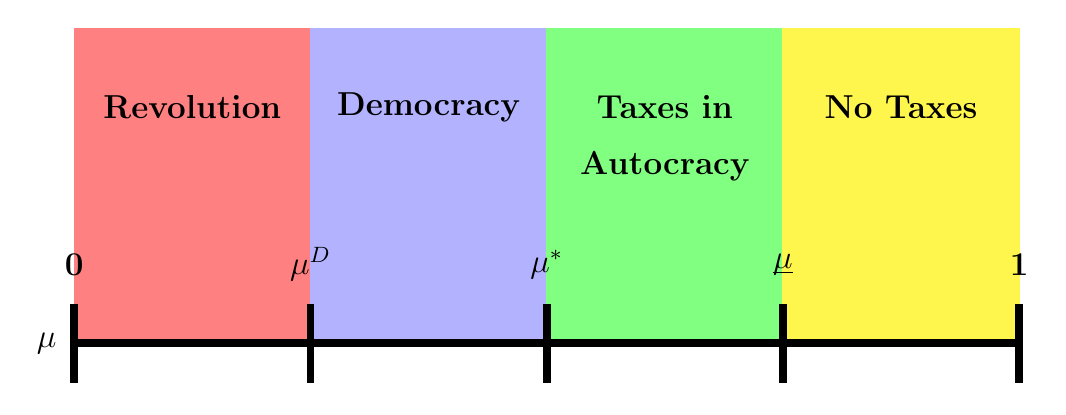
\begin{tikzpicture}	
		\draw[draw = red!50,fill=red!50] (-2,0) -- (1,0) -- (1,4) -- (-2,4) -- (-2,0);
		\draw[draw= blue!30,fill=blue!30] (1,0) -- (4,0) -- (4,4) -- (1,4) -- (1,0);
		\draw[draw=green!50, fill=green!50] (4,0) -- (7,0) -- (7,4) -- (4,4) -- (4,0);
		\draw[draw= yellow!70,fill = yellow!70] (7,0) -- (10,0) -- (10,4) -- (7,4) -- (7,0);
		\node[very thick,align=center,black] (r4) at (4,1)  {\large{$\mu^{*}$}};
		\draw[line width = 1mm] (4,.5) -- (4,-.5);
		\node[very thick,align=center,black] (r4) at (7,1)  {\large{$\mathbf{\underbar{\ensuremath{\mu}}}$}};
		\draw[line width = 1mm] (7,.5) -- (7,-.5);
		\node[very thick,align=center,black] (r4) at (1,1)  {\large{$\mu^{D}$}};
		\draw[line width = 1mm] (1,.5) -- (1,-.5);
		\node[very thick,align=center,black] (r4) at (5.5,3)  {\large{\bf Taxes in}};
		\node[very thick,align=center,black] (r4) at (5.5,2.25)  {\large{\bf Autocracy}};
		\node[very thick,align=center,black] (r4) at (8.5,3)  {\large{\bf No Taxes}};
		\node[very thick,align=center,black] (r4) at (2.5,3)  {\large{\bf Democracy}};
		\node[very thick,align=center,black] (r4) at (-0.5,3)  {\large{\bf Revolution}};
		\draw[line width = 1mm] (-2,0) -- (10,0);
		\draw[line width = 1mm] (-2,.5) -- (-2,-.5);
		\draw[line width = 1mm] (10,.5) -- (10,-.5);
		\node[very thick,align=center,black] (r4) at (-2.35,0) {\large{$\mu$}};
		\node[very thick,align=center,black] (r4) at (-2,1) {\large{\bf 0}};
		\node[very thick,align=center,black] (r4) at (10,1) {\large{\bf 1}};
	\end{tikzpicture}	
	\end{center}
\end{figure}
